\documentclass[../../../main_math.tex]{subfiles}

\begin{document}
\renewcommand{\col}{\geo}
\begin{multicols}{2}[\section{Algebraic topology}]
  	\subsection{Homotopy and fundamental group}
  	\subsubsection{Homotopy between maps and spaces}
  	
  	\begin{definition}
	  	Let $X,Y$ be two topological spaces \footnote{From now on $X$, $Y$ and $Z$ will always be topological spaces} and let $f,g: X \to Y$ be two continuous maps. A \emph{homotopy} between $f$ and $g$ is a continuous map $H:X\times [0,1] \to Y$ such that for all $x\in X$
	  	\begin{enumerate}
		  		\item $H(x,0)=f(x)$
		  		\item $H(x,1)=g(x)$.
		\end{enumerate}
		We say that $f$ and $g$ are \emph{homotopic} if there exists a homotopy between them, and we denote it by $f\simeq g$.
	\end{definition}
	  
	\begin{lemma}
	    Let $X=A\cup B$, where $A$ and $B$ are closed sets. If $\varphi: A \to Y$ and $\psi: B \to Y$ are continuous maps such that $\left.\varphi \right|_{A\cap B}=\left.\psi \right|_{A\cap B}$, then the map $$x\mapsto \begin{cases}
	    	\varphi(x) & \quad\text{if  } x\in A \\
	    	\psi(x)  & \quad\text{otherwise}\\
		\end{cases}$$ is also continuous.
	\end{lemma}
	
	\begin{proposition}
		The relation $\simeq$ is an equivalence relation between continuous maps.
    \end{proposition}
		
	\begin{definition}
		A continuous map $f:X\to Y$ is called a \emph{homotopy equivalence} if there exists a map $g:Y\to X$ such that $f\circ g\simeq id_Y$ and $g\circ f \simeq id_X$. We say that $X$ and $Y$ are \emph{homotopy equivalent} or that they have the same \emph{type of homotopy} if there exists a homotopy equivalence between them, and we denote it by $X\simeq Y$.
	\end{definition}

  	\begin{proposition}
		The relation $\simeq$ is an equivalence relation between topological spaces.
	\end{proposition}

	\begin{definition}
		A space having the homotopy type of a point is called\emph{contractible}.
	\end{definition}
	
	\subsubsection{Paths and foundamental group}
	
	\begin{definition}
		A \emph{path} in $X$ is a continuous map $\sigma:[0,1]\to X$.
	\end{definition}

	\begin{definition}
		Let $\sigma, \tau : [0,1]\to X$ be two paths such that $\sigma(0)=\tau(0)$ and $\sigma(1)=\tau(1)$. A homotopy between them is a continuous map $H:[0,1]\times [0,1] \to X$ such that
		\begin{enumerate}
			\item $H(s,0)=\sigma(s) $ $\forall s\in [0,1]$
			\item $H(s,1)=\tau(s)$ $\forall s\in [0,1]$
			\item $H(0,t)=\sigma(0)=\tau(0)$ $\forall t\in [0,1]$
			\item $H(1,t)=\sigma(1)=\tau(1)$ $\forall t\in [0,1]$
		\end{enumerate}
	When there exists a homotopy between $\sigma$ and $\tau$ we say that they are \emph{homotopic}, and we write $\sigma \simeq \tau $.
	\end{definition}

	\begin{proposition}
		The relation $\simeq$ is an equivalence relation between paths.
	\end{proposition}

	\begin{definition}
		Let $\sigma, \tau: [0,1] \to X$ such that $\sigma(1)=\tau(0)$. We define the product of $\sigma, \tau$ as 
		\begin{align*}
			\sigma \cdot \tau: [0,1] &\longrightarrow X \\
			x&\longmapsto \begin{cases}
				\sigma(2s) & 0\leq s \leq \frac{1}{2}\\
				\tau(2s-1)  & \frac{1}{2}\leq s \leq 1\\
			\end{cases}.
		\end{align*}
	
	\end{definition}

	\begin{lemma}\label{ProdCamins}
		Let $\sigma, \sigma', \tau, \tau':[0,1]\to X$ be paths such that 
		\begin{enumerate}
			\item $\sigma(0)=\sigma'(0)$
			\item $\sigma(1)=\sigma'(1)=\tau(0)=\tau'(0)$
			\item $\tau(1)=\tau'(1)$.
		\end{enumerate}
		If $\sigma \simeq \sigma'$ and $\tau \simeq \tau'$ then $\sigma \cdot \tau \simeq \sigma' \cdot \tau'$.
	\end{lemma}

	%IMATGE DE CAMINS?
	
	\begin{definition}
		A \emph{loop at the basepoint $x_0$} is a path $\sigma: [0,1]\to X$ such that $\sigma(0)=\sigma(1)=x_0$.
	\end{definition}

	\begin{definition}
		The \emph{foundamental group} of $X$ at the basepoint $x_0$ is the set of all homotopy classes of loops at the basepoint $x_0$, and it is denoted by $\pi_1 (X,x_0)$. We define $[\sigma]\cdot [\tau]:=[\sigma \cdot \tau]$, which is well-defined by \cref{ProdCamins}.
	\end{definition}

	\begin{proposition}
		$\big(\pi_1(X,x_0), \cdot \big)$ is a group.
	\end{proposition}
	
	\begin{proposition}
		Let $x_0, y_0 \in X$. If there exists a path $\gamma: [0,1] \to X$ from $x_0$ to $y_0$ then $\pi_1 (X,x_0) \cong \pi_1 (X,y_0)$.
	\end{proposition}
	
	\begin{proof}
		\begin{align*}
			\varphi: \pi_1(X,x_0) &\longrightarrow \pi_1(X,y_0) \\
			[\sigma]&\longmapsto [\gamma \cdot \sigma \cdot \gamma^{-1}]\\
		\end{align*}
		is an isomorphism.
	\end{proof}
	
	\begin{definition}
		Let $f:X\to Y$ be a continuous map, and $x_0 \in X$. We define 
		\begin{align*}
			f_*: \pi_1 (X,x_0) & \longrightarrow \pi_1 (Y,f(x_0)) \\
			[\alpha] &\longmapsto [f\circ \alpha].
		\end{align*}
		
	\end{definition}

	\begin{proposition}
		Let $f,g:X\to Y$ and $h:Y \to Z $ be continuous maps. Then
		\begin{enumerate}
			\item $f_*$ is well-defined and it is a group morphism.
			\item If $f\simeq g$ and $f(x_0)=g(x_0)$, then $f_*=g_*$.
			\item $(h\circ f)_*=h_*\circ f_*$.
		\end{enumerate}
	\end{proposition}

	\begin{corollary}
		$X\simeq Y \implies \pi_1 (X,x_0) \cong \pi_1 (Y,f(x_0))$.
	\end{corollary}

	%EXPLICAR RELACIO ENTRE HOMOTOPIES I GRUPS AMB DIAGRAMES


	\subsubsection{Foundamental group of $S^1$}
	
	\begin{lemma}
		Let (X,d) be a compact metric space, and $\{U_1, ..., U_n\}$ a finite cover of open sets of $X$. Then there exists $\varepsilon>0$ such that $\forall x \in X$, $B(x,\varepsilon)\subset U_i$ for some $i$. Such a number $\varepsilon$ is called a Lebesgue number of the cover.
	\end{lemma}

	\begin{proof}
		Let $C_i=X\setminus U_i$.  Then the map 
		
		\begin{align*}			
			f:X &\longrightarrow [0, +\infty) \\
			x &\longmapsto \frac{1}{n} \sum d(x,C_i)			
		\end{align*}
		
		is a continuous map on a compact set and therefore reaches the minimum at $X$. $\varepsilon=\min f$ satisfies the desired properties.
	\end{proof}
	
	\begin{lemma}
		Let $\sigma: [0,1] \to S^1$ be a loop such that $\sigma(0)=(1,0)$. Then, there is a unique path $\tilde{\sigma}: [0,1] \to \mathbb{R}$ such that $\tilde{\sigma}(0)=0$ and $\operatorname{exp}\circ\tilde{\sigma}=\sigma$, where $\operatorname{exp}(x)=\exp{2\pi x i}$. Such a path $\tilde{\sigma}$ is called a \emph{lift} of $\sigma$. Morover, if $\sigma \simeq \tau$ then $\tilde{\sigma}(1)=\tilde{\tau}(1)$.
	\end{lemma}
	\begin{proof}
		Let $U=S^1\setminus\{(1,0)\}$ and $V=S^1\setminus\{(-1,0)\}$. Let $k\in \mathbb{N}$ be such that $1/k<\varepsilon$, where $\varepsilon$ is a Lebesgue number of the cover $\{\sigma^{-1}(U), \sigma^{-1}(V)\}\subset [0,1]$. For every $n\in \mathbb{N}$ $\operatorname{exp}: (n,n+1)\to U$ and $\operatorname{exp}: (n-\frac{1}{2},n+\frac{1}{2})\to V$ are homeomorphisms and, therefore, for every $1\leq i \leq k$ there exists unique $\tilde{\sigma}_i: [\frac{i-1}{k}, \frac{i}{k}]\to \mathbb{R}$ such that $\operatorname{exp}\circ\tilde{\sigma_i}=\sigma|_{[\frac{i-1}{k}, \frac{i}{k}]}$, and $\tilde{\sigma}_{i+1}(\frac{i}{k})=\tilde{\sigma}_i(\frac{i}{k})$ if $i\geq 1$ and $\tilde{\sigma}_{1}(0)=0$. Finally, for $t\in[\frac{i-1}{k}, \frac{i}{k}]$ we define $\tilde{\sigma}(t)=\tilde{\sigma}_i(t)$. Now let's suppose that $H:[0,1]\times[0,1]\to S^1$ is a homotopy between $\sigma$ and $\tau$. A very similar argument shows that there exists continuous map $\tilde{H}:[0,1]\times[0,1]\to \mathbb{R}$ such that $\operatorname{exp}\circ \tilde{H}=H$. Thus, $t\mapsto \tilde{H}(1,t)$ is an integer-valued continuous map and, therefore, constant, which means that $\tilde{\sigma}(1)=\tilde{H}(1,0)=\tilde{H}(1,1)=\tilde{\tau}(1)$.
	\end{proof}
	
	\begin{theorem}
		The foundamental group of $S^1$ is isomorphic to $\mathbb{Z}$
	\end{theorem}
	
	\begin{proof}
		\begin{align*}
			\varphi: \pi_1(S^1, (1,0)) &\longrightarrow \mathbb{Z} \\
			[\sigma]&\longmapsto \tilde{\sigma}(1) \\
		\end{align*}
		is a well-defined isomorphism.
	\end{proof}
	
	\begin{definition}
		Let $A\subseteq X$ be a subspace of $X$. A \emph{retraction} of $X$ onto $A$ is a continuous map $r: X \to A$ such that $r(a)=a$ for all $a\in A$. If such a retraction exists, $A$ is called a \emph{retract} of $X$. 
	\end{definition}

	\begin{corollary}
		$S^1\subseteq \mathbb{D}^2$ is not a retract of $\mathbb{D}^2$.
	\end{corollary}

	%PROVA AMB DIAGRAMES

	\begin{theorem}[Brower 1910]
		\label{Brower}
		Every continuous map $f:\mathbb{D}^2 \to \mathbb{D}^2$ has a fixed point. 
	\end{theorem}

	\begin{proof}
		
		\begin{minipage}{0.3\textwidth}
			If $f(x)\neq x$ for every $x\in \mathbb{D}^2$, then the map $r: \mathbb{D}^2 \to S^1$ defined by $r(x)$ being the intersection of the line passing through $x$ and $f(x)$ and $S^1$ is a retraction of $\mathbb{D}^2$ to $S^1$.
		\end{minipage}
		\begin{minipage}{0.2\textwidth}
			\begin{center}
				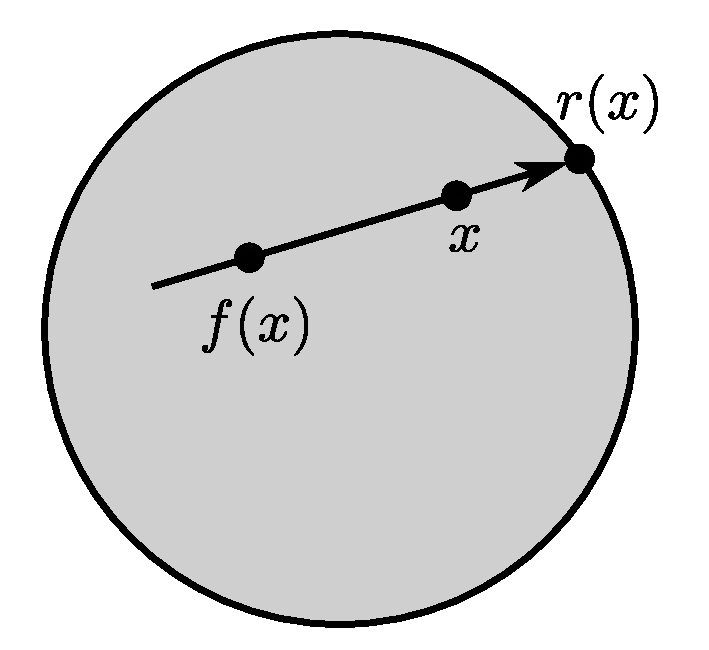
\includegraphics[width=0.6\textwidth]{Images/Brower.pdf}
			\end{center}
		\end{minipage}

	\end{proof}
	
	

	\begin{theorem}[Borsuk-Ulam]
		If $f:S^2 \to \mathbb{R}^2$ is a continuous map, then there exists $x\in S^2$ such that $f(x)=f(-x)$.
	\end{theorem}
	
	
\end{multicols}
\end{document}